\documentclass{article}
\usepackage{booktabs}
\usepackage{array}
\usepackage{wrapfig}
\usepackage{multirow}
\usepackage{tabularx}
\usepackage{graphicx}
\usepackage{amsmath}
\usepackage{amssymb}
\usepackage{mdframed}
\usepackage{polyglossia}
\setdefaultlanguage{english}
\usepackage[style=alphabetic,minalphanames=3,maxbibnames=99]{biblatex}
\usepackage{hyperref}
\addbibresource{references.bib}

\def\bitcoinA{%
  \leavevmode
  \vtop{\offinterlineskip %\bfseries
    \setbox0=\hbox{B}%
    \setbox2=\hbox to\wd0{\hfil\hskip-.03em
    \vrule height .3ex width .15ex\hskip .08em
    \vrule height .3ex width .15ex\hfil}
    \vbox{\copy2\box0}\box2}}

\newtheorem{definition}{Definition}[section]

\title{WabiSabi - Draft v0.3}
\author{Ádám Ficsór, Yuval Kogman, István András Seres}
\date{\today}

\begin{document}

\maketitle

\begin{abstract}
  Bitcoin's model for value transfer is a publicly verifiable ledger of transactions, with ownership of coins defined in terms of public keys. Although this design lacks strong guarantees for privacy, it does not rule it out.
  Despite the potential for private use, research has shown that users' activity can often be traced in practice.
  This lack of inherent privacy has given rise to business models built on dragnet surveillance of Bitcoin users which is problematic for Bitcoin's fungibility.

  A number of methods have been proposed to mitigate these issues. Among these, CoinJoin is an approach to structuring transactions which adds ambiguity and breaks common assumptions that underlie heuristics used for surveillance.
  Current implementations of CoinJoin transactions present a number of limitations which may partly explain their lack of widespread adoption.

  This work introduces a new protocol for centrally coordinated CoinJoin implementations utilizing keyed verification anonymous credentials and homomorphic value commitments. This is an improvement on the state of the art in both privacy and flexibility, enabling additional use cases and reduced overheads.
\end{abstract}

\section{Introduction}

Bitcoin transactions redistribute funds by consuming as inputs the outputs of previous transactions, and creating new outputs. The protocol rules enforced by the network ensure that transactions do not arbitrarily inflate the monetary supply and that outputs are spent at most once. While some newer cryptocurrencies use more sophisticated approaches to defining such rules, in Bitcoin the amounts as well as the specific outputs being spent are broadcast in the clear as part of the transaction. This presents significant challenges for transacting with privacy\footnote{In this work we restrict the discussion of Bitcoin privacy to that of transactions, but there are other considerations especially at the network layer. For a more comprehensive discussion see \url{https://en.bitcoin.it/wiki/Privacy}.} as shown already in some of the earliest academic studies of Bitcoin~\cite{ron2013quantitative,meiklejohn2013fistful,moser2013anonymity}.

The conditions for spending an output are specified in its \texttt{scriptPubKey}, typically requiring that the spending transaction be signed by a specific public key. The signatures authorizing a transaction usually commit to the transaction in its entirety, which makes it possible for mutually distrusting parties to jointly create transactions without risking misallocation of funds: participants will only sign a proposed transaction after confirming that their desired outputs are included.

Chaumian CoinJoin~\cite{mizrahi2013blind}\cite{maxwell2013coinjoin}\cite{zerolink} is a privacy enhancing technique that uses this atomicity property and Chaumian blind signatures~\cite{chaum1983blind} to construct collaborative Bitcoin transactions, also known as CoinJoins. Participants connect to a server, known as the coordinator, and submit their inputs and outputs using different anonymity network identities. This ensures anonymity, but on its own would allow users to disrupt the protocol by claiming a greater output amount than they registered as inputs. To mitigate this the coordinator provides blind signatures representing standard denominations in response to inputs, and output registration is allowed by presenting a valid signature without the coordinator being able to link the signature to a specific input.

The use of standard denominations in the resulting CoinJoin transaction obscures the relationship between individual inputs and outputs, making the origins of each output ambiguous. Unfortunately standard denominations also present limitations, such as requiring change outputs from these CoinJoin transactions, and limiting the usefulness of the privacy enhanced outputs for payments of arbitrary amounts.

\subsection{Limitations of ZeroLink}
In this work, we are aiming to improve ZeroLink, the most popular Chaumian CoinJoin implementation for Bitcoin. We identify several privacy shortcomings and inefficiencies of the current protocol as implemented by Wasabi. Some metrics comparing Wasabi, Samourai and other apparent CoinJoin transactions are provided. ``Other'' includes JoinMarket, but also has an inherent false positive error given these transactions are identified heuristically.

\subsubsection{Round denominations}

Due to the nature of blind signatures, mixed outputs of ZeroLink CoinJoins are restricted to a fixed set of value denominations which are multiples of a base denomination\footnote{approximately $0.1$\bitcoinA{}}.

This creates friction when sending or receiving arbitrary amounts of Bitcoin, as the fixed denomination generally creates change which is smaller, both when mixing and when spending mixed outputs.

We define \emph{CoinJoin inefficiency} as the fraction of non-mixed outputs in a CoinJoin transaction, see Figure~\ref{fig:cjinefficiency}.

\begin{figure}[h!]
    \centering
    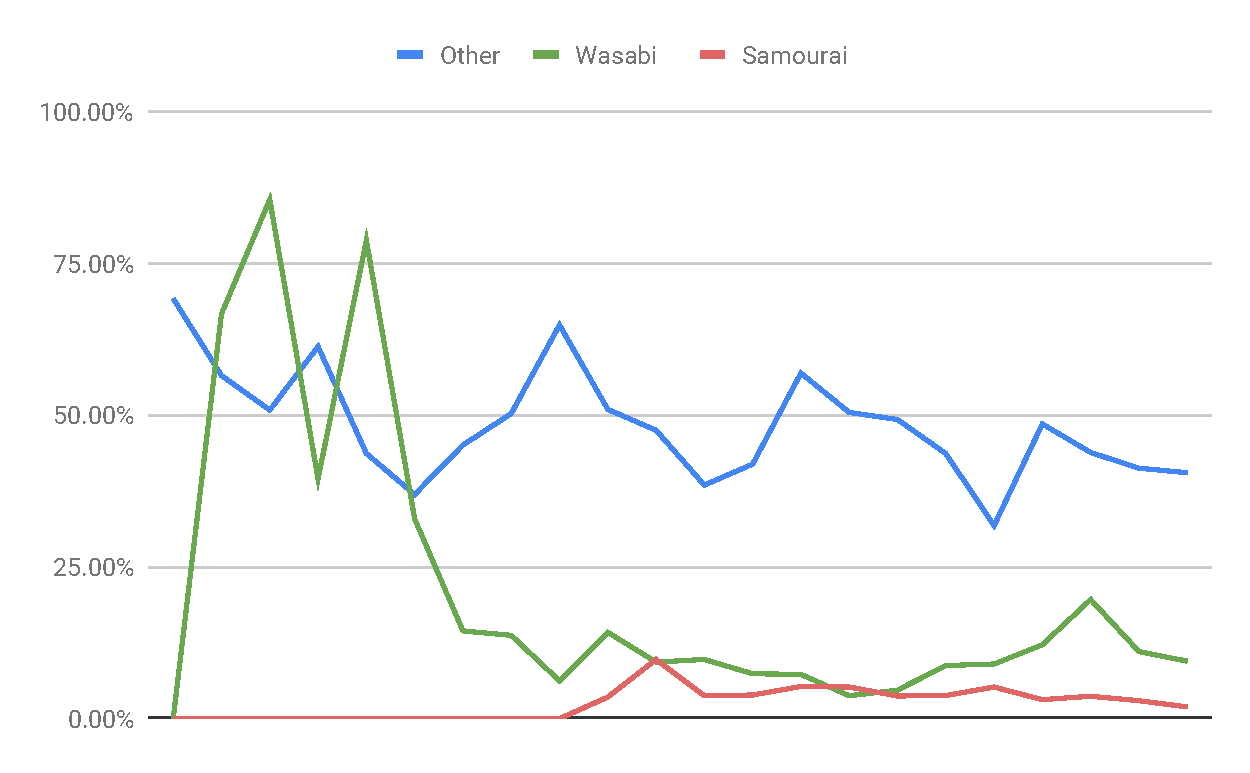
\includegraphics[scale=0.4]{Figures/CJInefficiency.pdf}
    \caption{CoinJoin inefficiency of various privacy-focused Bitcoin wallets}
    \label{fig:cjinefficiency}
\end{figure}

\subsubsection{Minimum denomination}

In order to pariticpate a user's combined input amount must be greater or equal to the base denomination. We observe, that considerable portion of CoinJoin inputs are less than this minimum denomination, see Figure~\ref{fig:minimumdenomination}.

\begin{figure}[h!]
    \centering
    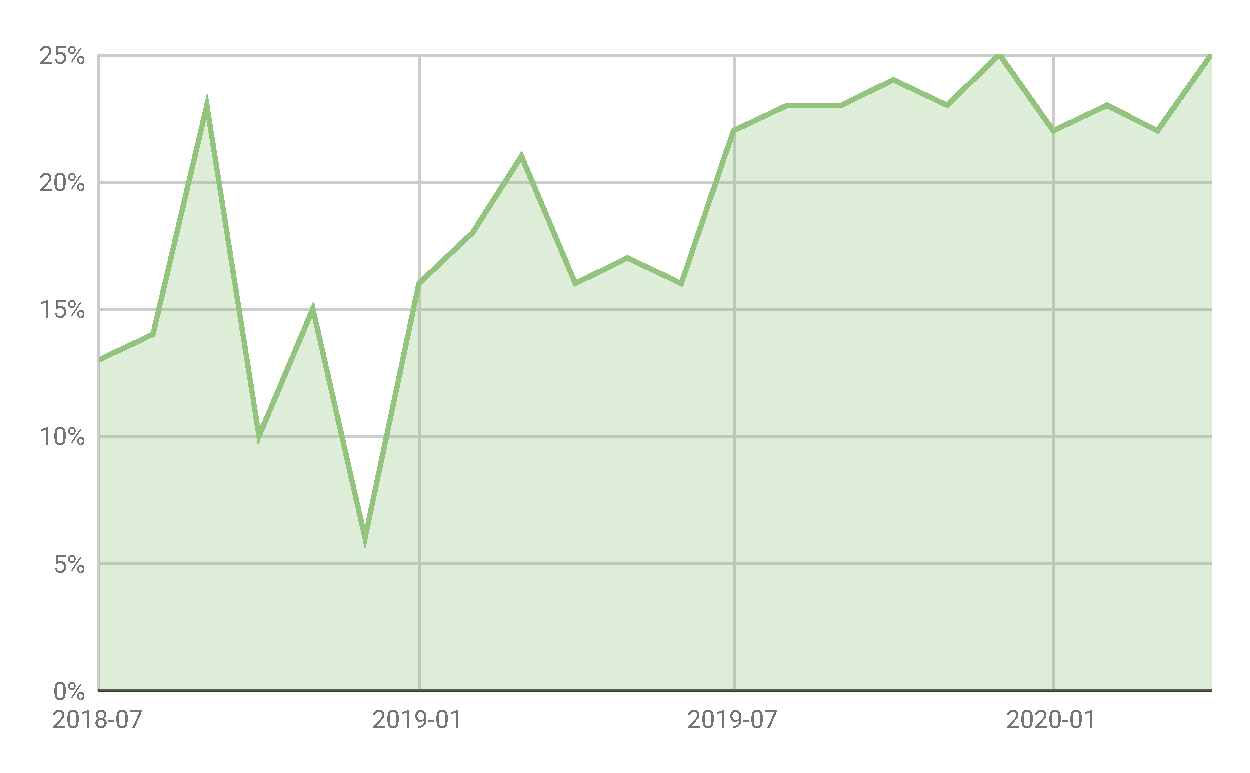
\includegraphics[scale=0.4]{Figures/SmallValueInputsWasabi.pdf}
    \caption{Fraction of input UTXOs with value smaller than the minimum denomination in Wasabi CoinJoin transactions}
    \label{fig:minimumdenomination}
\end{figure}

Even if users are able to provide several smaller value input UTXOs with total value greater than the minimum denomination, the coordinator knows those input UTXOs belong to the same user.  In an ideal mixing protocol the coordinator should not obtain more information than the already available blockchain data by coordinating the CoinJoin transaction.

Furthermore if users consolidate their UTXOs before the CoinJoin in an additional transaction in order to be able to participate in a CoinJoin, then this link is revealed publicly based on the common input ownership heuristic~\cite{meiklejohn2013fistful}.

\subsubsection{Variable denominations} Since users pay mining and coordination fees the denominations are gradually reduced between rounds in order to make it possible for users to mix several times without providing additional inputs. This introduces a perverse incentive to minimize coordination fees by remixing in quick succession in order, resulting in a smaller anonymity set than with time-staggered remixes.

\subsubsection{Block-space efficiency}

The rigidity of the current ZeroLink transaction structure, i.e. fixed denominations, constrains users' UTXO set structure as well. These limitations force users to consolidate their UTXOs (see Figure~\ref{fig:postmixmerging}) and create additional interemdiate outputs with constrained amounts when interspersing CoinJoin transactions with transactions that send or receive value.

\begin{figure}[h!]
    \centering
    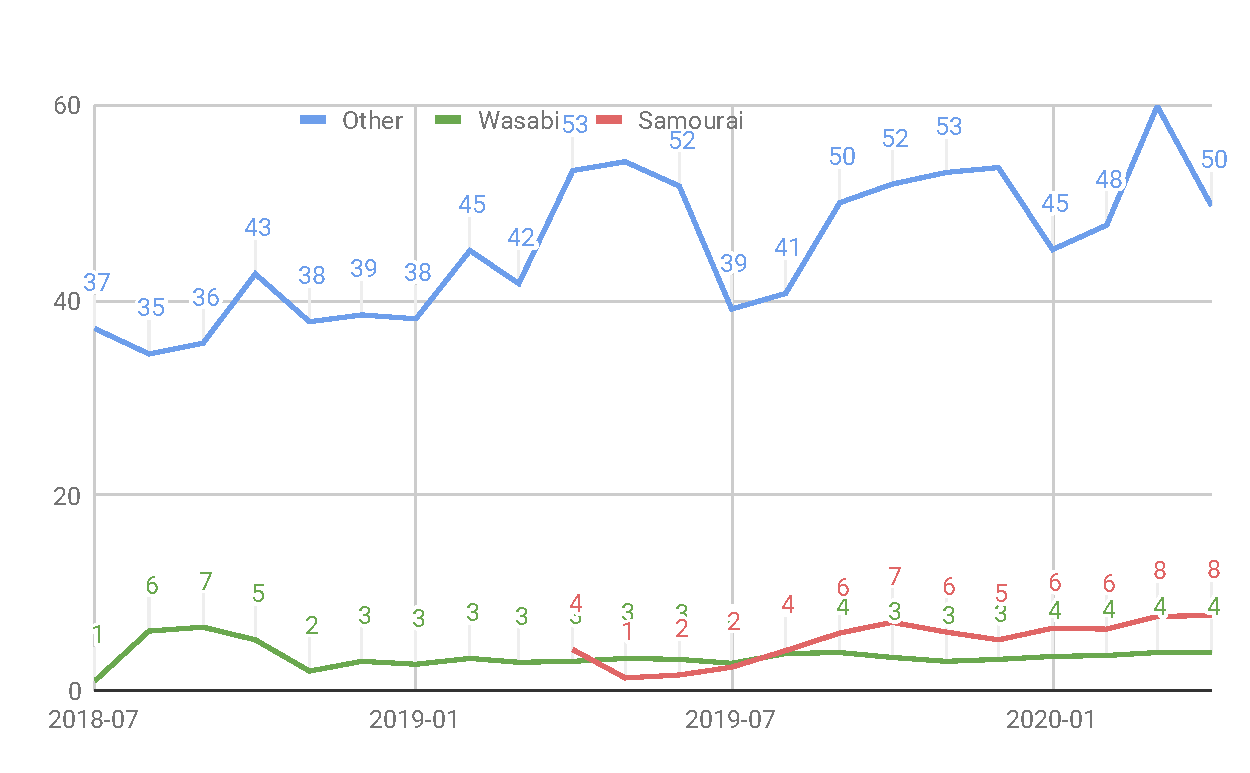
\includegraphics[scale=0.4]{Figures/postMixInputMerging.pdf}
    \caption[]{Average number of inputs from the first post-mix transactions in various CoinJoin schemes.\footnotemark}
    \label{fig:postmixmerging}
\end{figure}

\footnotetext{The high numbers of consolidation of other CoinJoin like transactions suggest the algorithm used to identify them yielded a large number of false positive results.}

\subsubsection{Lack of privacy-enhanced payments} Currently ZeroLink supports neither payments from a CoinJoin, nor payments in a CoinJoin. Payments from a CoinJoin would protect sender privacy and improve efficiency by requiring fewer intermediate outputs. Payments within a CoinJoin would protect both sender and receiver privacy, and since it is a form of PayJoin~\cite{payjoin} would also improve privacy since it introduces degrees of freedom in the interpretation of CoinJoins.

\subsection{Our Contribution}

We introduce WabiSabi, a generalization of Chaumian CoinJoin based on a Keyed-Verification Anonymous Credentials-based (KVAC) scheme~\cite{chase2019signal}. The use of KVACs replaces blind signatures' standard denominations with homomorphic amount commitments, similar to Confidential Transactions~\cite{maxwell2016confidential}, but retains the invariant that the sum of any one participant's outputs does not exceed that of their inputs without the coordinator learning the underlying values. In addition to being more flexible this improves privacy compared to standard denominations, since smaller inputs can be combined and change outputs created with the same unlinkability guarantees as the privacy enhanced outputs\footnote{Note that the cleartext amounts appearing in the final transaction might still link individual inputs and outputs.}.

WabiSabi can be instantiated to construct a variety of CoinJoin transaction structures that depart from the standard output denomination convention, such as SharedCoin and CashFusion~\cite{cashfusion} style transactions and Knapsack~\cite{maurer2017anonymous} mixing. Additionally it makes possible arbitrary consolidation of outputs, minimizing unmixed change, relaxing minimum required denominations, improved block space efficiency, making payments from CoinJoins, as well as payments within CoinJoins, also known as PayJoins~\cite{payjoin}.

\section{Preliminaries}

Hereby we give an informal and high-level description of applied cryptographic primitives. In the following the security parameter is denoted as $\lambda$.

\subsection{Commitment schemes}
A commitment scheme allows a party to commit to a message without enabling them to change their mind about the committed message after publishing the commitment. On the other hand the commitment should not reveal anything about the committed message.

\noindent$\mathsf{Commit}(m,r)\xrightarrow{}\mathcal{C}$. The $\mathsf{Commit}$ algorithm generates a commitment $\mathcal{C}$ to message $m$ using randomness $r$.

\noindent$\mathsf{OpenCom}(\mathcal{C},m,r)\xrightarrow{}\{\mathit{True},\mathit{False}\}$: one can verify the correctness of the opening of a commitment by checking $\mathcal{C}\stackrel{?}{=}\mathsf{Commit}(m,r)$. If equality holds the algorithm outputs $\mathit{True}$, otherwise $\mathit{False}$.

For ease of understanding the reader can assume in the following that the commitment scheme is instantiated as a Pedersen commitment.

\subsection{MAC}
A message authentication code (MAC) ensures the integrity of a message and consists of the following three probabilistic polynomial-time algorithms.

\noindent$\mathsf{GenMACKey}(\lambda)\xrightarrow{}{\mathsf{sk}}$. a party generates a secret key $\mathsf{sk}$ for MAC generation and verification.

\noindent$\mathsf{MAC}_{\mathsf{sk}}(m)\xrightarrow{}t$. one can generate a MAC $t$ on a message a $m$ by using their $\mathsf{sk}$.

\noindent$\mathsf{VerifyMAC}_{\mathsf{sk}}(m,t)\xrightarrow{}\{\mathit{True},\mathit{False}\}$. The issuer of the MAC can verify a MAC $t$ given the message $m$ it was issued on.

The reader might intuitively think of a MAC as the symmetric-key counterpart of digital signatures. They both have the same goals and similar security requirements, however a MAC is not publicly verifiable.

\subsection{Zero-knowledge proofs of knowledge}
A very high-level, and hence somewhat imprecise, description of zero-knowledge proofs is provided. This protocol involves a prover and a verifier. A prover wishes to prove that a relation $\mathcal{R}$ holds with respect to a secret input $w$, called witness, and public input $x$. Specifically, the prover wants to prove that $(x, w) \in \mathcal{R}$ without revealing anything about $w$.

\noindent$\mathsf{Prove}(x,w,\mathcal{R})\xrightarrow{}\pi$. Given $x$ and the private witness $w$ the prover generates a proof $\pi$.

\noindent$\mathsf{Verify}(x,\pi,\mathcal{R})\xrightarrow{}\{\mathit{True},\mathit{False}\}$. The verifier is given the proof $\pi$ and $x$ and decides whether the prover knows a secret $w$ such that $\mathcal{R}(x,w)=1$ holds.

\section{Protocol Overview}

\subsection{Terminology and notation}

\begin{definition} \textbf{Credential}:
An anonymous credential is issued by the coordinator at input registration, and certifies attributes that the coordinator validates before issuing. The user can then prove possession of a valid credential in zero-knowledge in order to register an output without the coordinator being able to link it to the input registration from which it originates, or any other output registrations.

We use keyed-verification anonymous credentials (introduced in~\cite{chase2014algebraic}), in particular the scheme from~\cite{chase2019signal} which supports group attributes (attributes whose value is an element of the underlying group $\mathbb{G}$). We instantiate this scheme with two group attributes.
\end{definition}

\begin{definition}\textbf{Attribute}:
In order to facilitate construction of Bitcoin transactions, our credentials represent confidential Bitcoin amounts. For this we use two attributes: $M_v$ is a commitment to the amount of the registered input in satoshis and $M_s$ is a commitment to a serial number used for double spending prevention.

During credential presentation randomized versions of the attributes are presented, which we denote $C_v$ and $C_s$.
\end{definition}

Finally, $k$ is a protocol level constant, denoting the number of credentials used in input and output registration requests, and $v_{\mathit{max}} = 2^{51}-1$ constrains the amount value ranges.\footnote{$\log_2(2099999997690000) \approx 50.9$}

\subsection{Phases}

A CoinJoin round consists of an Input Registration, an Output Registration and a Transaction Signing phases. To defend against Denial of Service attacks it is important to ensure the inputs of users who do not comply with the protocol are identified, thus these inputs can be excluded from the following rounds in order to ensure completion of the protocol.

\begin{enumerate}
    \item While identifying non-compliant inputs during Input Registration phase is trivial, there is no reason for issuing penalties at this point.
    \item Identifying non-compliant inputs during Output Registration phase is not possible, thus this phase always completes and progresses to the Signing Phase.
    \item During Signing Phase, inputs those do not sign are non-compliant inputs and they shall be issued a penalties.
\end{enumerate}

The point of the cryptography in WabiSabi is to ensure it does not worth for any non-compliant input to sign the final CoinJoin transaction, otherwise non-compliant inputs could not be identified. We achieve this by ensuring no user can register outputs those sum is larger than its registered inputs' sum.

\subsection{Registration}

For intuition we first we describe a pair of naive protocols for input and output registration, followed by a generalization into a unified protocol described in detail in \S\ref{details}.

\subsubsection{Input Registration}

The user, acting as Alice, submits an input of value $v_{\mathit{in}}$ along with $k$ pairs of group attributes,
$(M_{v_i}, M_{s_i})$.
She proves in zero knowledge that the sum of the requested sub-amounts is equal to $v_{\mathit{in}}$ and that the individual amounts are positive integers in the allowed range.

The coordinator verifies the proofs, and issues $k$ MACs on the requested attributes, along with a proof of knowledge of the secret key as described in \textit{Credential Issuance} protocol of \cite{chase2019signal}.

\begin{figure}
    \begin{mdframed}
    \begin{enumerate}
        \item Alice sends $k$ credential requests with accompanying range and sum proofs to the coordinator:  $((M_{v_i},M_{s_i},\pi^{\textit{range}}_{i})^{k}_{i=1},\pi^{sum},v_{\textit{in}})$.
        \item The coordinator verifies the received proofs. If they are not verified, coordinator aborts the protocol, otherwise issues $k$ MACs on the requested attributes $(\mathsf{MAC}_\mathsf{sk}(M_{v_i},M_{s_i}), \pi_i^{\mathrm{iparams}})^{k}_{i=1}$.
    \end{enumerate}

\end{mdframed}
    \caption{Input Registration protocol}
    \label{fig:inputreg}
\end{figure}

\subsubsection{Output Registration}

Now acting as Bob, to register her output the user randomizes the attributes and generates a proof of knowledge of $k$ valid credentials issued by the coordinator.

Additionally, she proves knowledge of representation of the serial number commitments. These serial numbers are revealed for double spending protection, but the knowledge of commitment opening should be done in zero knowledge to avoid revealing the randomness of the original commitment in the input registration phase or the randomization added in output registration time.

Finally, Bob proves that the sum of her randomized amount attributes $C_v$ matches the requested output amount $v_{\mathit{out}}$, analogously to input registration.\footnote{Note that there is no need for range proofs, since amounts have been previously validated}

She submits these proofs, the randomized attributes, and the serial numbers. The coordinator verifies the proofs, and if it accepts the output will be included in the transaction.

\begin{figure}[h]
    \begin{mdframed}
    \begin{enumerate}
        \item Bob sends $k$ randomized commitments, a proof of a valid MAC for the corresponding non-randomized commitments, the underlying serial numbers with a proof of the representation of their commitments, and finally a proof of the sum of the amounts:   $((C_{v_i},C_{s_i},\pi_{i}^{\textit{MAC}},s_i, \pi_i^{\textit{serial}})^{k}_{i=1}, \pi^{\textit{sum}}, v_{\textit{out}})$.
        \item The coordinator verifies proofs and registers requested output iff. all proofs are valid and the serial numbers have not been used before.
    \end{enumerate}
\end{mdframed}
    \caption{Output Registration protocol}
    \label{fig:outputreg}
\end{figure}

\subsubsection{Unified Registration}

For more flexibility in a dynamic setting, where a user may not yet know her desired output allocation during input registration, and to allow for small\footnote{Specifically, $2 \le k \le 10 \approx \log_2\left(\frac{\mathtt{MAX\_STANDARD\_TX\_WEIGHT} - 58}{274 + 124}\right)$, because although $k=1$ suffices for flexibility it limits parallelism, leaking privacy by temporal fingerprinting.} values of $k$, we can generalize input and output registration into a single unified protocol, which also supports reissuance.

In this case Alice or Bob (depending on the registration phase) submits $k$ valid credentials and $k$ credential requests, where the sums of the underlying amount commitments must be balanced.

To prevent the coordinator from being able to distinguish between initial vs. subsequent input registration requests (which may merge amounts) registration operations credential presentation should be mandatory. Initial credentials can be obtained with an auxiliary bootstrapping operation.

\begin{figure}[h]
  \begin{mdframed}
    \begin{enumerate}
    \item During input registration phase Alice submits $k$ credential requests:  $(M_{v_i},M_{s_i},\pi^{\mathit{null}}_{i})^{k}_{i=1}$
    \item The coordinator verifies the received proofs. If it accepts, it issues $k$ MACs on the requested attributes $(\mathsf{MAC}_\mathsf{sk}(M_{v_i},M_{s_i}), \pi_i^{\mathrm{iparams}})^{k}_{i=1}$.
    \end{enumerate}
  \end{mdframed}
  \caption{Credential bootstrapping protocol}
  \label{fig:bootstrap}

    \begin{mdframed}
    \begin{enumerate}
        \item During input (output) registration phase, Alice (Bob, resp.) submits:
        \begin{itemize}
            \item $k$ credential requests with accompanying range and sum proofs to the coordinator:  $(M_{v_i},M_{s_i},\pi^{\textit{range}}_{i})^{k}_{i=1}$
            \item $k$ randomized commitments, a proof of a valid credential for the corresponding non-randomized commitments, the underlying serial numbers and a proof of the representation of their commitments: $(C_{v_i},C_{s_i},\pi_{i}^{\mathit{MAC}},s_i,\pi_i^{\textit{serial}})^{k}_{i=1}$
            \item A balance proof: $(\pi^{\textit{sum}}, \Delta_{v})$
            \item If $\Delta_{v} \ne 0$, an input or output with value $|\Delta_{v}|$.
        \end{itemize}
        \item The coordinator verifies the received proofs, and that the serial numbers have not been used before, and depending on the current phase, $\Delta_{v} \geq 0$ (input) or $\Delta_{v} \leq 0$ (output). If it accepts, it issues $k$ MACs on the requested attributes $(\mathsf{MAC}_\mathsf{sk}(M_{v_i},M_{s_i}), \pi_i^{\mathrm{iparams}})^{k}_{i=1}$, and if $\Delta_{v} \ne 0$, registers the input or output with value $|\Delta_{v}|$.
    \end{enumerate}
    \end{mdframed}
    \caption{Unified Registration protocol}
    \label{fig:reissue}
\end{figure}


\subsection{Signing phase}

The user fetches the finalized but unsigned transaction as Satoshi, and if she sees her registered outputs she will sign, submitting the signature as Alice(s).

\section{Cryptographic Details}\label{details}

Following \cite{chase2019signal}, the scheme is defined in a group \(\mathbb{G}\) of prime order \(q,\) written in multiplicative notation.
$\mathsf{HashTo\mathbb{G}} : {0,1}^* \mapsto \mathbb{G}$ is a function from strings to group elements, based on a cryptographic hash function.

We require the following fixed set of group elements for use as generators with different purposes:
\[
\underbrace{G_{w}, G_{w^{\prime}}, G_{x_{0}}, G_{x_{1}}, G_{V}}_{\mathsf{MAC} \text{~and~} \mathsf{Show}}
\qquad
\underbrace{G_{v}, G_{s}}_{\text{attributes}}
\qquad
\underbrace{G_g, G_h}_{\text{commitments}}
\]
chosen so that nobody knows the discrete logarithms between any pair of them, e.g. $G_h = \mathsf{HashTo\mathbb{G}}(``\texttt{h}")$.

This notation deviates slightly from \cite{chase2019signal}, in that we subscript the attribute generators $G_{y_i}$ as $G_v$ and $G_s$ instead of using numerical indices, and we require two additional generators $G_g$ and $G_h$ for constructing the attributes $M_v$ and $M_s$ as Pedersen commitments.

As with the generator names, we modify the names of the attribute related components of the secret key
$\mathrm{sk} = (w, w^{\prime}, x_{0}, x_{1}, y_{v}, y_{s}) \in_R {\mathbb{Z}_q}^6$
according to our fixed set of group attributes.

The coordinator parameters
$\mathit{iparams} =  (C_{W}, I)$
are computed as:
\[
C_{W}={G_w}^{w} {G_{w^\prime}}^{w^\prime}
\quad
I=\frac{G_{V}}{{G_{x_0}}^{x_0} {G_{x_1}}^{x_1} {G_{y_v}}^{y_v} {G_{y_s}}^{y_s}}
\]
These are used by the coordinator to prove correctness of issued MACs, and by the users to prove knowledge of a valid MAC.

\subsection{Credential Requests}

For each $i \in [1, k]$ the user chooses an amount $0 \leq v_i < v_{\mathit{max}}$ subject to the constraints of the balance proof (\S\ref{balance}) and a serial number $s_i \in_R \mathbb{Z}_q$.

She commits to these with randomness $r_{v_i}, r_{s_i} \in_R \mathbb{Z}_q$, and these commitments are the attributes of the requested credentials.:
\[ M_{v_i}={G_g}^{r_{v_i}}{G_h}^{v_i} \qquad M_{s_i}={G_g}^{r_{s_i}}{G_h}^{s_i} \]

For each amount $v_i$ she also computes a range proof which ensures there are no negative values:
\[
\pi^{\mathit{range}}_i = \operatorname{PK}\left\{\left(v_i, r_{v_i} \right) :
M_{v_i} = {G_g}^{r_{v_i}}{G_h}^{v_i}
\land
0 \leq v_i < v_{\mathit{max}} \right\}
\]

We note that if Bulletproofs~\cite{bunz2018bulletproofs} are utilized for the range proofs $\pi^{\textit{range}}_i$ a single combined proof will significantly decrease the communication overhead.

For initial credential requests the range proofs can be replaced with simpler proofs of $v_i = 0$:
\[
  \pi^{\mathit{null}}_i = \operatorname{PK}\left\{ \left( r_{v_i}\right) :
    M_{v_i} = {G_{g}}^{r_{v_i}}
  \right\}
\]

\subsection{Credential Presentation}

The user is in possession of $k$ credentials with a valid MAC obtained from prior registration requests.

For each credential $i \in [1, k]$ she executes a modified version of the $\mathsf{Show}$ protocol described in~\cite{chase2019signal}:

\begin{enumerate}

\item She chooses
$z_i \in_{R} \mathbb{Z}_{q}$, and computes
$z_{0_i}=-{t_i} {z_i} (\bmod q)$
and the randomized commitments:
\begin{align*}
C_{v_i}     &= {G_v}^{z_i} M_{v_i} \\
C_{s_i}     &= {G_s}^{z_i} M_{s_i} \\
C_{x_{0_i}} &= {G_{x_0}}^{z_i} {U_i} \\
C_{x_{1_i}} &= {G_{x_1}}^{z_i} {U_i}^{t_i} \\
C_{V_i}     &= {G_V}^{z_i} V_i
\end{align*}

\item To prove to the coordinator that a credential is valid she computes a proof:
\begin{align*}
\pi_{i}^{\mathit{MAC}}=\operatorname{PK}\{
& (z_i, z_{0_i},t_i): \\
& Z_i =I^{z_i} \land \\
& C_{x_{1_i}} = {C_{x_{0_i}}}^{t_i} {G_{x_0}}^{z_{0_i}} {G_{x_1}}^{z_i} \}
\end{align*}
which implies the following without allowing the coordinator to link $\pi_{i}^\mathit{MAC}$ to the underlying attributes $(M_{v_i}, M_{s_i})$:
\[
\mathsf{Verify}((C_{x_{0_i}}, C_{x_{1_i}}, C_{V_i}, C_{v_i}, C_{s_i}, Z_i), \pi_i^{\mathit{MAC}})
\iff
\mathsf{VerifyMAC}_{\mathsf{sk}}(M_{v_i}, M_{s_i})
\]

\item She sends $(C_{x_{0_i}}, C_{x_{1_i}}, C_{V_i}, C_{v_i}, C_{s_i}, \pi_i^{\mathit{MAC}})$ and the coordinator computes:
\[
Z_i=\frac{C_{V_i}}{{G_w}^w {C_{x_{0_i}}}^{x_0} {C_{x_{1_i}}}^{x_{1}}
{C_{v_i}}^{y_v} {C_{s_i}}^{y_s}
}
\]
using its secret key (independently of the user's derivation), and verifies $\pi_i^{\mathit{MAC}}$.

\end{enumerate}

\subsection{Over-spending prevention by balance proof}\label{balance}

The user needs to convince the coordinator that the amounts redeemed and the amounts requested differ by $\Delta_{v}$, which she can prove by including the following witness-hiding proof:
\[ \pi^{\mathit{sum}}=\left( \sum_{i=1}^{k} r_{v_i}, \sum_{i=1}^k z_i\right) \]

During the input registration phase $\Delta_{v}$ may be positive, in which case an input of amount $v_{\mathit{in}} = \Delta_{v}$ must be registered with proof of ownership. During the output registration phase $\Delta_{v}$ may be negative, in which case an output of amount $v_{\mathit{out}} = -\Delta_{v}$ is registered. If $\Delta_{v} = 0$ credentials are simply reissued, with no input or output registration occurring.

\[ \prod_{i=1}^{k} \frac{M_{v_i}}{C_{v_i}}
\stackrel{?}{=}
\frac{ {G_g}^{\pi^{\mathit{sum}}[1]}{G_h}^{\Delta_{v}} }{ {G_v}^{\pi^{\mathit{sum}}[2]} }
\]

% remove? rewrite?
%Note that this equality over the product of the commitments implies the following  equality of the sum of the amounts is correct:
%\[\prod_{i=1}^{k} M_{v_i}
%= {G_g}^{\sum_{i=1}^{k} r_{v_i}} {G_h}^{\sum_{i=1}^{k} v_i}
%\iff
%\sum_{i=1}^{k} v_i = v_{\mathit{in}}
%\]

Informally soundness of the proof system holds as user does not know the discrete logs between the generator points used in the randomized commitments. Zero knowledge with respect to the witnesses is ensured since $\sum_{i=1}^{k}z_i$ does not leak anything about individual $z_i$. We can have a similar argument for $\sum_{i=1}^{k}r_{v_i}$ and $r_{v_i}$.

\subsection{Double-spending prevention using serial numbers}

The user proves knowledge of representation of her submitted randomized serial number commitments, namely:
\[ \pi_{i}^{\mathit{serial}}=\operatorname{PK}\{ (z_i, r_{s_i}): C_{s_i} = {G_s}^{z_i}{G_g}^{r_{s_i}}{G_h}^{s_i} \} \]
where the serial number $s_i$ is a public input, revealed to prevent double spending.

The coordinator verifies the $\pi_{i}^{\mathit{serial}}$ and checks that the $s_i$ have not been used before (allowing for idempotent registration).

\subsection{Credential Issuance}

If the coordinator accepts all of the above, it registers the input or output if one is provided, and for each $i \in [1,k]$ it issues a credential by responding with
$(t_i, U_i, V_i) \in \mathbb{Z}_q \times \mathbb{G} \times \mathbb{G}$,
which is the output of
$\mathsf{MAC}_{\mathsf{sk}}(M_{v_i}, M_{s_i})$,
where:
\[
t_i \in_{R} \mathbb{Z}_{q}, U_i \in_{R} \mathbb{G}
\qquad
V_i={G_w}^{w} {U_i}^{x_{0}+x_{1} t_i}{M_{v_i}}^{y_v} {M_{s_i}}^{y_s}
\]

To rule out tagging of individual users the coordinator must prove knowledge of the secret key, and that $(t_i, U_i, V_i)$ is correct relative to $\mathit{iparams}=(C_{W}, I)$:

\begin{align*}
\pi_{i}^{\mathit{iparams}}=\operatorname{PK}\{ & (w, w^{\prime}, x_{0}, x_{1}, y_v, y_s): \\
&C_{W}={G_{w}}^{w} {G_{w^{\prime}}}^{w^\prime} \land \\
&I=\frac{G_{V}}{{G_{x_{0}}}^{x_0} {G_{x_1}}^{x_1} {G_{y_v}}^{y_v} {G_{y_s}}^{y_s}} \land \\
&V_i={G_w}^{w}{U_i}^{x_{0}+x_{1}t_i} {M_{v_i}}^{y_v} {M_{s_i}}^{y_s}
\}
\end{align*}

\subsection{Perfect Hiding}

Note that after revealing $s_i$ we no longer have perfect hiding in the $M_{s_i}$ commitment, because there is exactly one $r_{s_i} \in \mathbb{Z}_q$ such that $M_{s_i} = {G_g}^{r_{s_i}} {G_h}^{s_i}$. Similarly, randomization by $z_i$ only protects unlinkability of issuance and presentation against a computationally bounded adversary.

To unconditionally preserve user privacy in the event that the hardness assumption of the discrete logarithm problem in $\mathbb{G}$ is broken we can add an additional randomness term $r_{s_i}^{\prime}$ used with an additional generator $G_g^{\prime}$ to the serial number commitments $M_{s_i}$, and similarly another randomness term $z_i^{\prime}$ and generators $G_v^{\prime}, G_s^{\prime}, G_{x_0}^{\prime}, G_{x_1}^{\prime}, G_V^{\prime}$ in order to obtain unconditional unlinkability for the commitments.\footnote{Assuming the coordinator is not able to attack network level privacy and the proofs of knowledge are unconditionally hiding.}

% TODO are the value commitments also an issue? what about for initial credentials where $M_{v_i} = G_g^{r_{v_i}}$? do we gain anything from having a single multi-commitment attribute?

\printbibliography

\end{document}
